\chapter{Collection and Analysis of Human Gait Data}
\label{chap:gaitdata}
\section{Introduction}

Marker-based motion capture systems(mocap) are popular methods of collecting biomechanical data. The body's movement can be tracked by placing markers on various locations on a person's body. These systems produce a significant amount of data, including marker positions, joint angles, and rigid body orientation. Additional sensors, such as Electromyography sensors (EMGs), force plates, and inertial measurement units (IMUs), can be added to measure muscle activity and joint torques. Marker-based trackers work by using several 2D cameras to track the 3D position of retro-reflective markers.  

Biomechanists and engineers use this data for kinematics, dynamics, and kinetics of human motion analysis, and to learn motion primitives of human motion \cite{10.7717/peerj.918}. It has been used for the assessment of orthosis \cite{kobetic2009development},  to analyze gait motion for people with lower-limb impairments \cite{lauer2005application} \cite{hicks2011lower}  \cite{cutler2015using} , and to learn and replicate human motion \cite{ott2008motion} \cite{chalodhorn2007learning}. 

The human leg is made of three joints; a hip, a knee and a ankle. The hip can be modeled has a ball and socket joint allowing for abduction/adduction, and transverse external/internal rotation \cite{faptakinesiology}. The knee is not a simple hinge joint, the tibia translate during flexion/extension rotation. It allow allows slight abduction/adduction and interail/external rotation. The knee is also responsible for taking loads during a gait cycle \cite{kuo2007six}. The ankle joint is synovial joint that helps absorb loads during a gait cycle. These joints are important for understanding the gait cycle.


\section{Motion Capture Trials}

One of the Motion Caption Trials goals is to collect enough data to mimic the motion of a healthy gait.  Despite how widely studied and researched the gait cycle and the numerous gait trials conducted, there is very little open-source raw data available, the most popular is the Winter $\it{et. al}$ database \cite{winter1991biomechanics}, yet this library only contains a few subjects. There are other gait data libraries available, but small and have additional restrictions for use. There is a need for additional data to be released for public use. The more data available, the better it helps to train robotics systems and develop exoskeletons and orthosis \cite{moore2015elaborate}. Additional gait and human motion data were collected and released open-source in Github \footnote{https://github.com/WPI-AIM/AIM\_GaitData} to solve this problem. The gait database comprises measurements of how gait varies from person to person when walking across the floor several times and climbing stairs of varying heights. 


\subsection{System setup}
\label{sec:setup}
The Vicon\footnote{Vicon Motion Systems Ltd, Oxford, UK}  Vantage V5 running at $100Hz$ was used to record the locomotion of a person. The system consisted of 10 cameras to track the position of the reflective markers. The makers were placed according to the plug-in gait lower limb template. Two AMTI \footnote{https://www.amti.biz/index.aspx} force plates were placed in the ground to record the joint dynamics. The force plates are synced to the Vicon through the Lock+ box \footnote{https://www.vicon.com/hardware/devices/lock/} running at $1000Hz$. \autoref{fig:markers} shows the placement of the markers on the legs of the subject. 



\begin{figure}
\centering 
\begin{subfigure}{0.4\linewidth} 
  \centering 
  \includegraphics[scale=0.05,frame]{images/gait_data/marker_side_cap.png} 
  \caption[Side Marker Placement]{Side few of the markers} 
  \label{fig:markers_side} 
\end{subfigure} 
%
\begin{subfigure}{0.4\linewidth} 
  \centering 
  \includegraphics[scale=0.05,frame ]{images/gait_data/front_markers_cap.png} 
  \caption[Front Marker Placement]{Front view of the markers} 
  \label{fig:markers_front} 
\end{subfigure} 
\caption[Marker Placement]{The markers were placed according to the plugin marker template. Additional rigid body plates were placed on the subjects' thighs, shanks, feet and back} 
\label{fig:markers} 

\end{figure} 

% \begin{figure}
%     \centering
%     \includegraphics{images/gait_data/marker_side_coor.png}
%     \caption{Marker position for gait collection}
%     \label{fig:gaitmarkerlayout}
% \end{figure}

Eleven able-bodied subjects participated in the study (5F, 6M). The Institutional Review Board of Worcester Polytechnic Institute approved the study, and each subject gave written consent. The data was anonymous, so the subjects could not be identified. \autoref{tab:subjects} holds the metadata of the subjects. All the data was saved in an ASCII format file. The custom open-source software package parses the data (\autoref{chap:software}).

\begin{table}[h!]
\centering
 \begin{tabular}{|c c c c c|} 
 \hline 
 \multicolumn{5}{|c|}{Subjects} \\
 \hline
 ID & Mass ($Kg$) &  Height($m$)  & Age($yr$)  & Gender \\ [0.5ex] 
 \hline\hline
 0 & 59 & 1.6 & 20 & F \\
 \hline
 1 & 62 & 1.7 & 20 & F \\ 
 \hline
 2 & 86 & 1.9 & 44 & F \\
 \hline
 3 & 64 & 1.8 & 20 & M \\ 
 \hline
 4 & 50 & 1.5 & 20 & F \\
 \hline
 5 & 96 & 1.6 &  19 & F\\
 \hline
 6 & 77 & 1.8 & 22 & M \\
 \hline
 7 & 78 & 1.8 & 22 & M \\
 \hline
 8 & 95 & 1.7 & 33 & M \\
 \hline
 9 & 85 & 1.8 & 21 & M \\
 \hline
 10 & 69 & 1.7 & 22 & M \\[1ex] 
 \hline
\end{tabular}
\caption[Subject Table]{The subject's meta data record at time of the trial.}
\label{tab:subjects}
\end{table}



 In the first task, the subjects walked approximately 3$m$ at their own pace and stride length \cite{peters2014concurrent}. The subjects were allowed to choose their leading leg. The subject walked across the floor three times to ensure that good data was collected. 

 In the second task, the subjects walked forward approximately 2$m$ and climbed three steps at their own pace. Markers were placed on each step of the staircase and on the floor to record their positions. The subjects approached the staircase, paused, and climbed the stairs with their leading leg. Each subject was allowed to climb at their own pace. Each subject repeated the action three times for each of the four different stairs of different heights, stair heights given in \autoref{tab:stairs}. The repetition of each subject ensured that a good sample trial with no marker occlusion was collected.   
 \begin{figure}[h]
    \centering 
    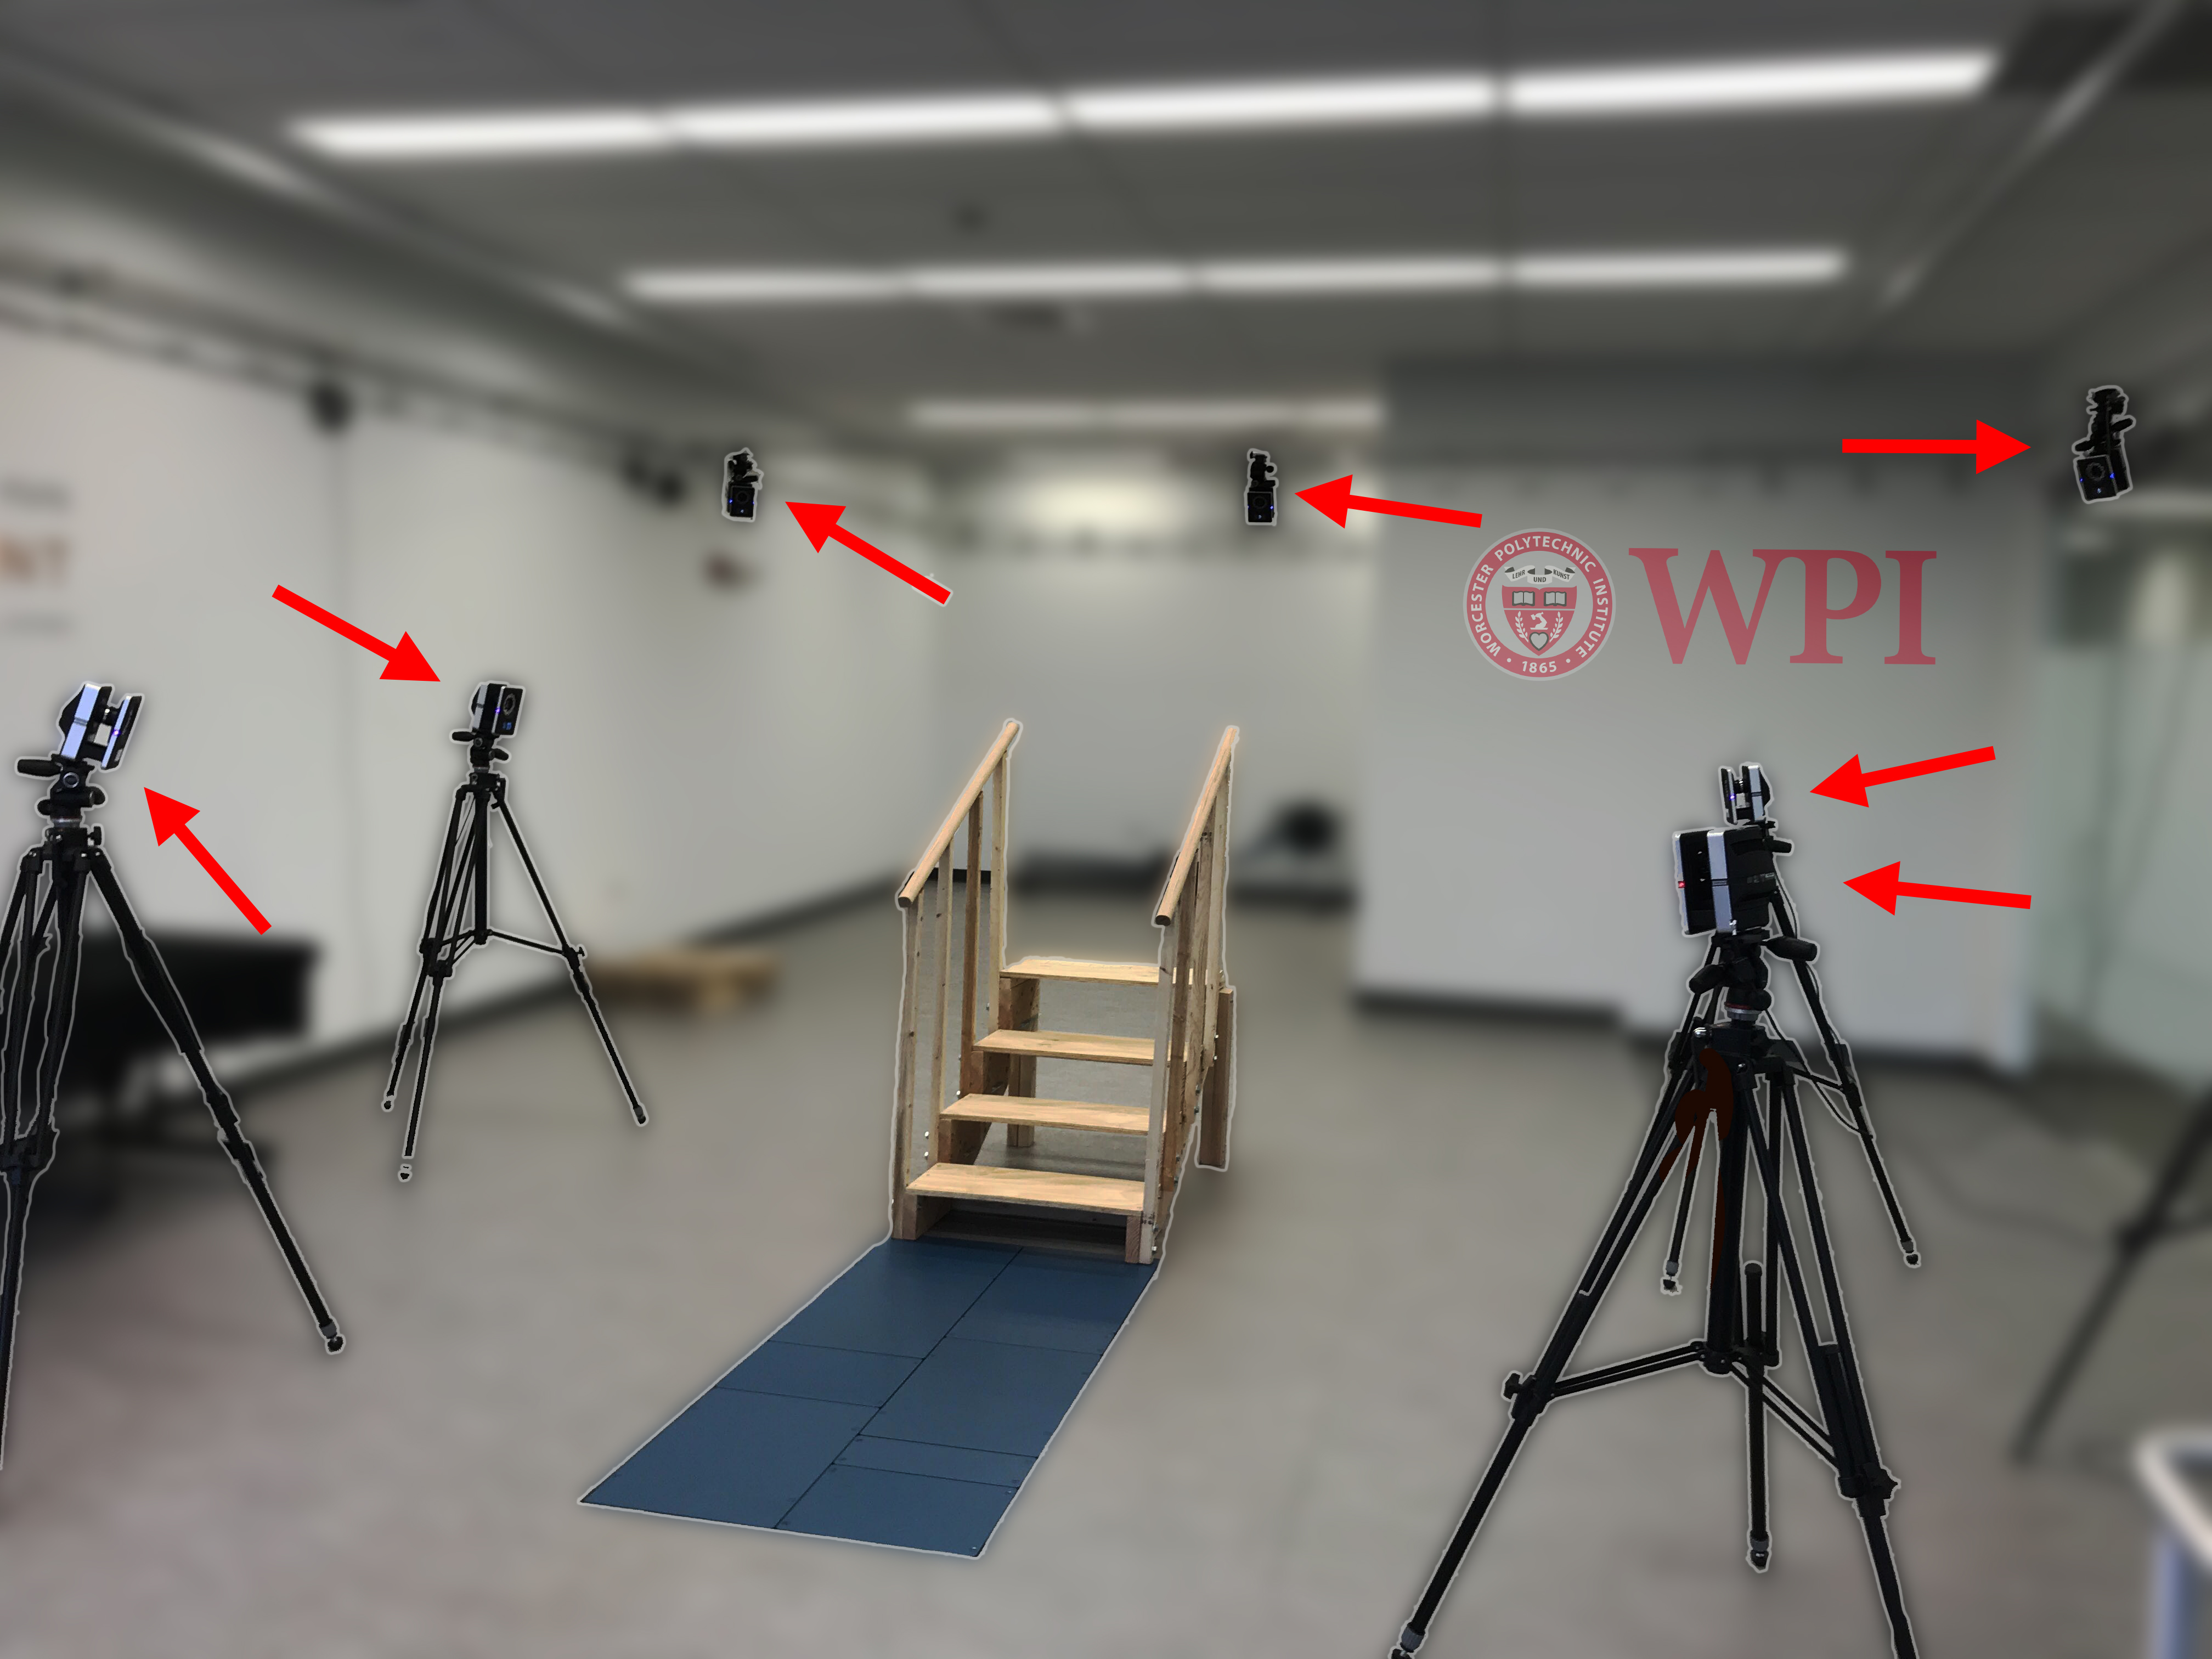
\includegraphics[scale=0.1,frame]{images/gait_data/stairs_EDIT.jpg}
    \caption[Motion Capture Area]{Motion capture area with custom staircases. The stairs had sliding planes to adjust the heights. Seven of the camera are shown and indicated with the green arrows and additional three camera are located off the image.  }
    \label{fig:mocap} 
\end{figure} 
 
\begin{table}[h!]
\centering
\large
 \begin{tabular}{||c c ||} 
 \hline
 Config & stair height (inch) \\ [0.5ex] 
 \hline\hline
 0 & 5.25  \\ 
 \hline
 1 & 6.0  \\
 \hline
 2 & 6.75  \\
 \hline
 3 & 7.5 \\
 \hline
\end{tabular}
\caption{Stair Height Configuration}
\label{tab:stairs}
\end{table}



\section{Analysis of Human Gait}

The goal of collecting the human motion data was to build a model for replicating the gait cycle to allow the exoskeleton to follow a natural joint motion. Using multiple demonstrations to train a stable estimation of a multi-dimensional dynamic system of nonlinear motion can be learned \cite{li2018development}. The mocap provides an abundance of data to study the motion of human movement. The individual marker location is used to learn the motion of a body segment. Since it is desired to generate a walking motion, the joint angles throughout the gait cycle create the training demonstrations.  A single gait cycle was extracted from each of the gait cycles,  \autoref{fig:TrainingDemosGait} shows the extracted gait cycles. Each of the lines represents a different subject. As expected, the gait cycles follow a similar trajectory with slight variation in starting and endpoints. 

\begin{figure}[h]
    \centering
    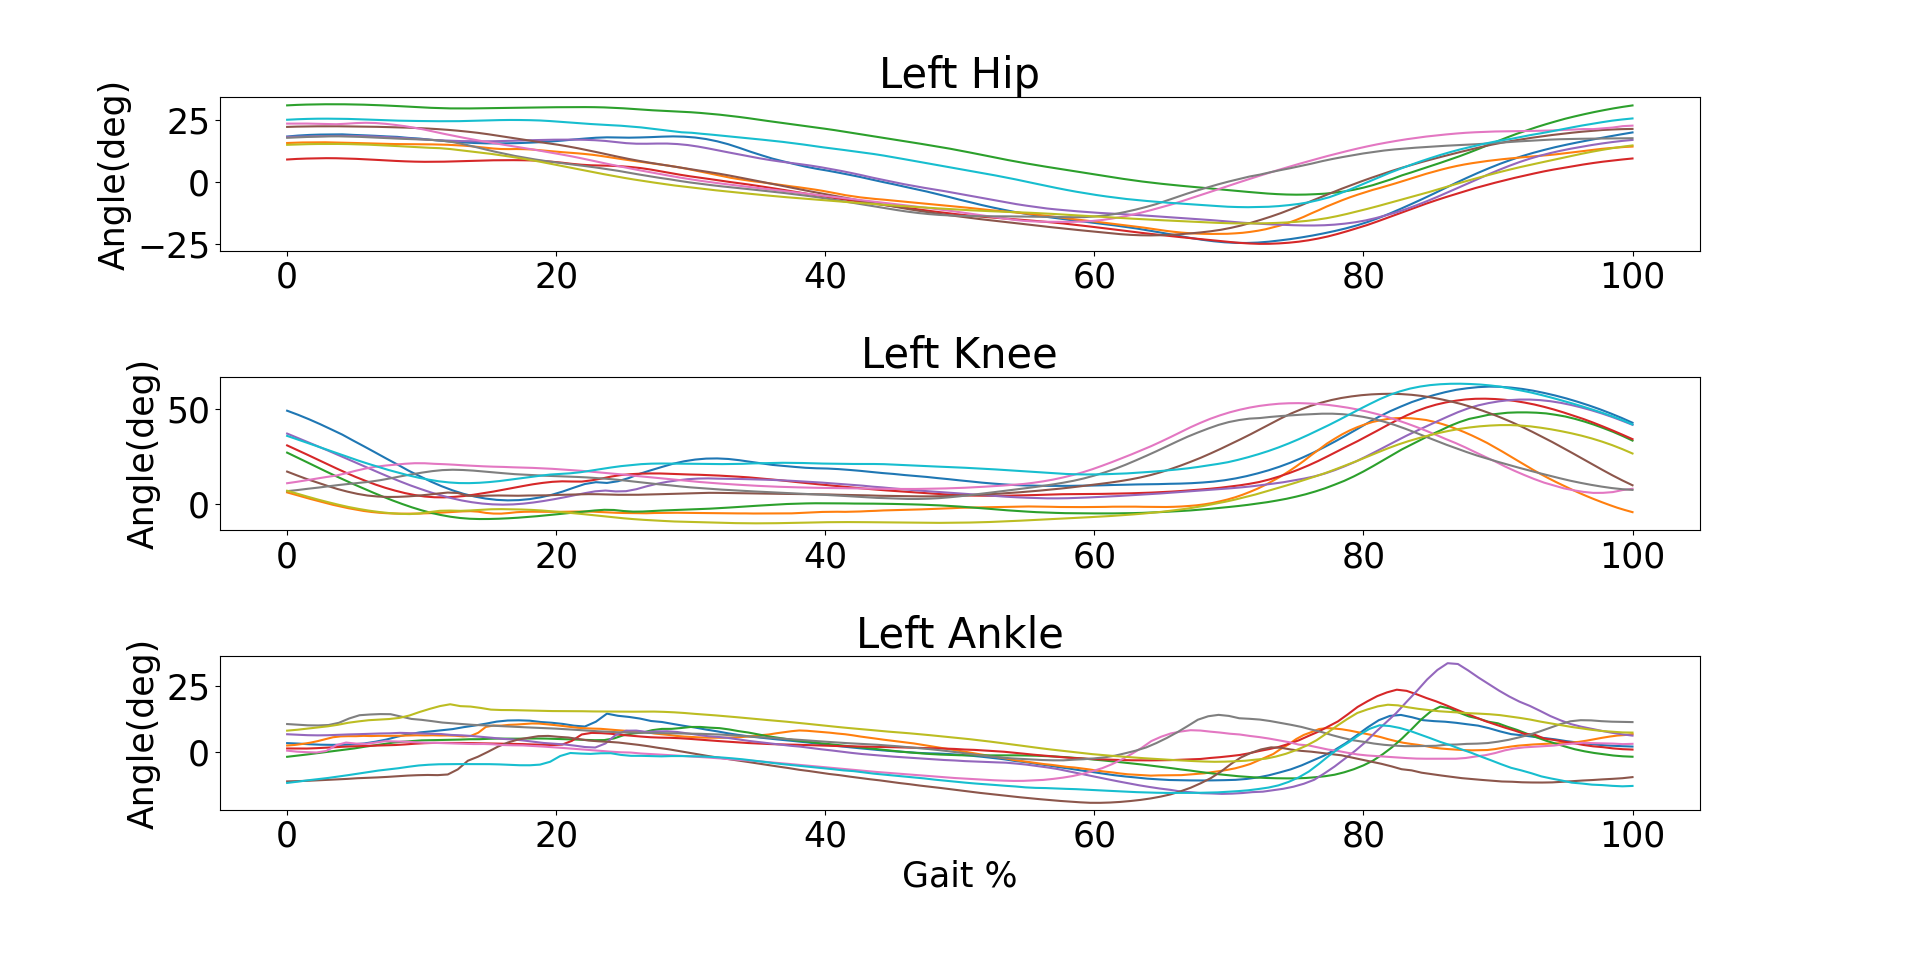
\includegraphics[scale=0.30]{images/gait_data/gaittraining.png}
    \caption[Neutral Joint With Markers]{Neutral Joint With Markers}
    \label{fig:TrainingDemosGait}
\end{figure}

\begin{figure}[h]
    \centering
    \includegraphics[scale=0.060]{images/gait_data/Joint_direction_mocap.png}
    \caption[Gait Training Demos]{Joint angle markers and joint angle direction}
    \label{fig:TrainingJointPosition}
\end{figure}

TPGMM (\autoref{eq:MstepTPGMM}, \autoref{eq:EstepTPGMM}) was used to learn the motion of the trajectory. This unsupervised learning method allows for the features of the motion to be extracted for encoding. This method has not been used for learning and implementing gait motions as discussed in \autoref{sec:applfd}.  The advantages of this method are the following:

\begin{itemize}
    \item Allows the use of natural gait motions instead of hand-coded motion.
    \item Temporal scaling of the trajectory allowing for gaits to be slowed down or speed up.
    \item Spatial scaling of the motion allowing for the start and goal positions.
    \item Principled approach for the distribution of the Gaussians.
    \item Provides mixture model parameters for measuring the variance along with the demonstrations.
\end{itemize}


The BIC score was calculated for bin size 10-30 using  \autoref{eq:BIC}; due to the randomization initialization, the score and optimal bin size vary slightly. \autoref{fig:BIC} shows the BIC score for the bins sizes. On average, the optimal number of bins converged around 15 bins and used to learn the walking model.    

\begin{figure}
    \centering
    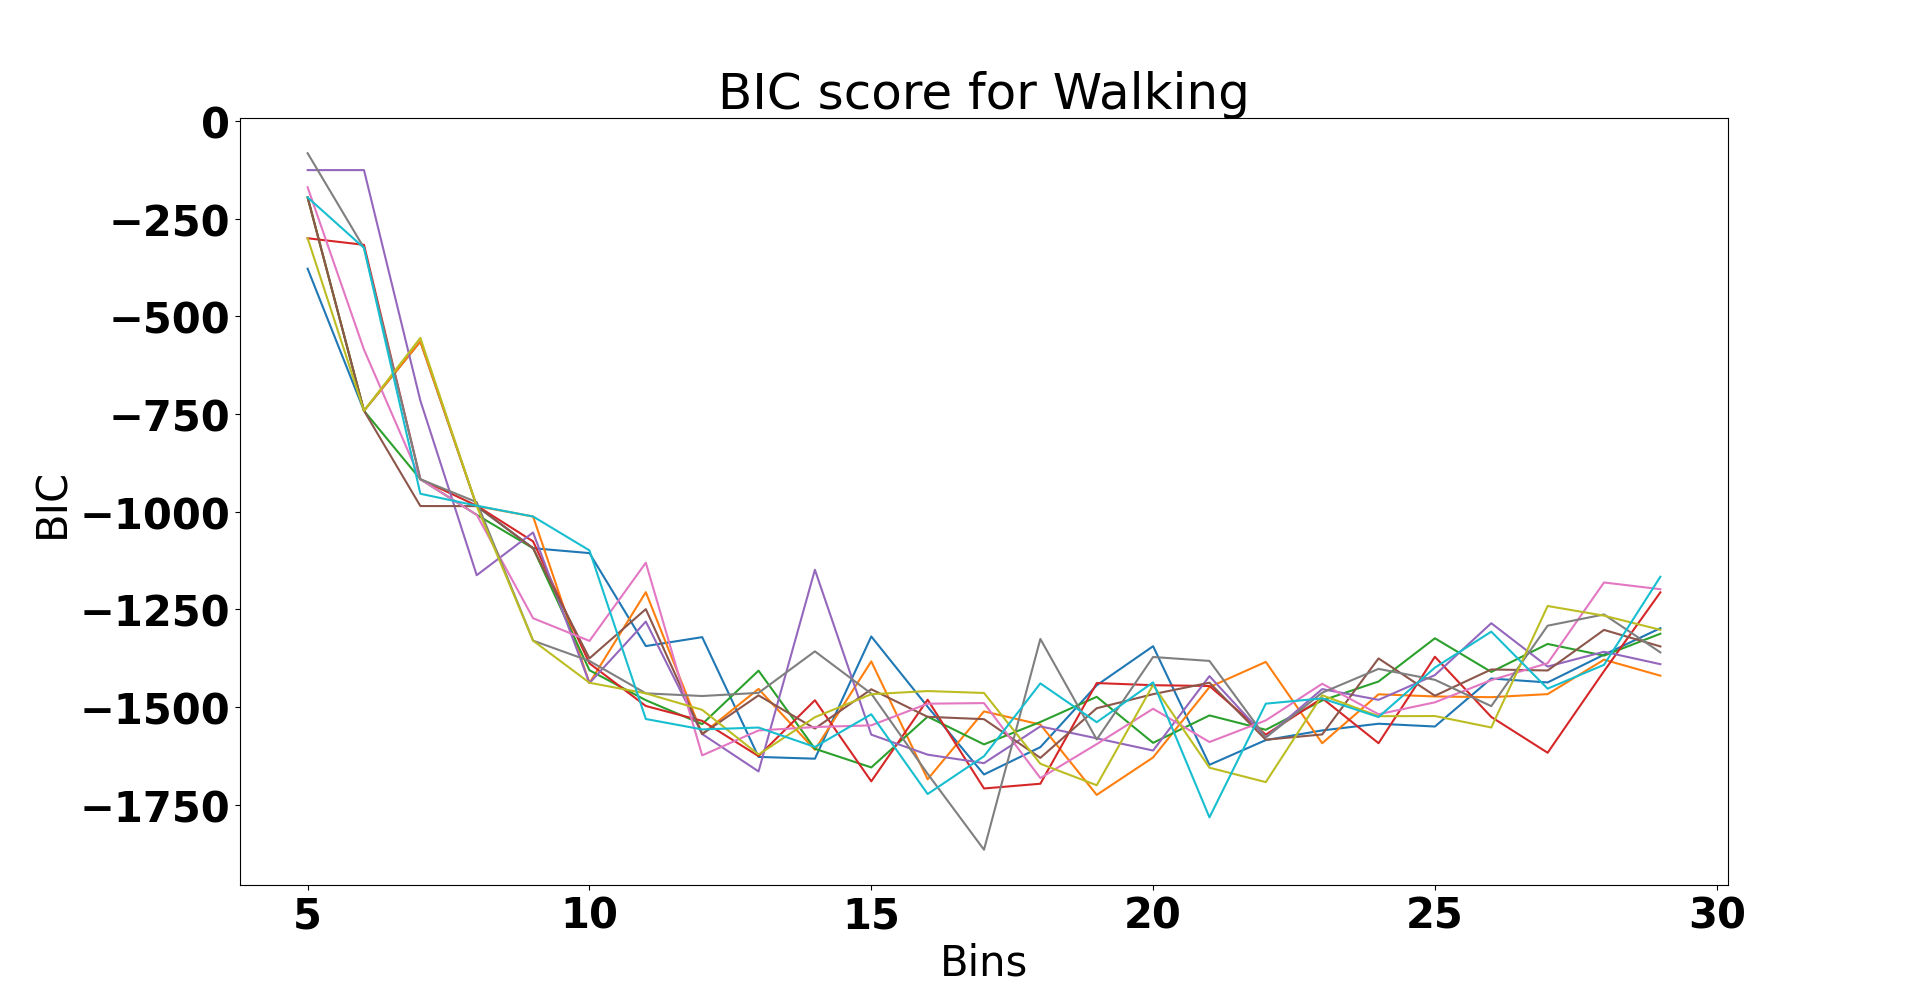
\includegraphics[scale=0.3]{images/gait_data/BIC_Walk.png}
    \caption[BIC score for walking]{The BIC score that determines the number of bins}
    \label{fig:BIC}
\end{figure}

The TPGMM process places the Gaussians that drive the system along the trajectory; this is shown in \autoref{fig:force}, the blue lines are the underline demonstrations transformed into a force.  The demonstrations were aligned using DTW. The red dots and green ovals are the means and covariances, and each oval is one of the bins (refer to \autoref{fig:cov_mat} for the calculations of the Gaussians).  GMR regresses over the means and covariances produced by the TPGMM process, accomplished through a superposition process of the overlapping Gaussians. The Gaussians with a smaller major and minor axis indicate a tight correlation, and the larger major and minor axis indicate less correlation of the points on the trajectory.  The Gaussians on the knee and ankle graphs have small variance along the demonstrations leading to small Gaussians. In contrast, the hip demonstrations have a more considerable variance leading to larger Gaussians. \autoref{fig:learnedModel} show the comparison of the learned model compared to the training demonstrations. The thin lines are the training demonstrations; the thick line is the trained model. The trajectories were extracted from the learned model above and used DMPs to reproduce each of the joints' trajectories. 


\begin{figure}[!h]
    \begin{subfigure}{\textwidth}
        \centering
        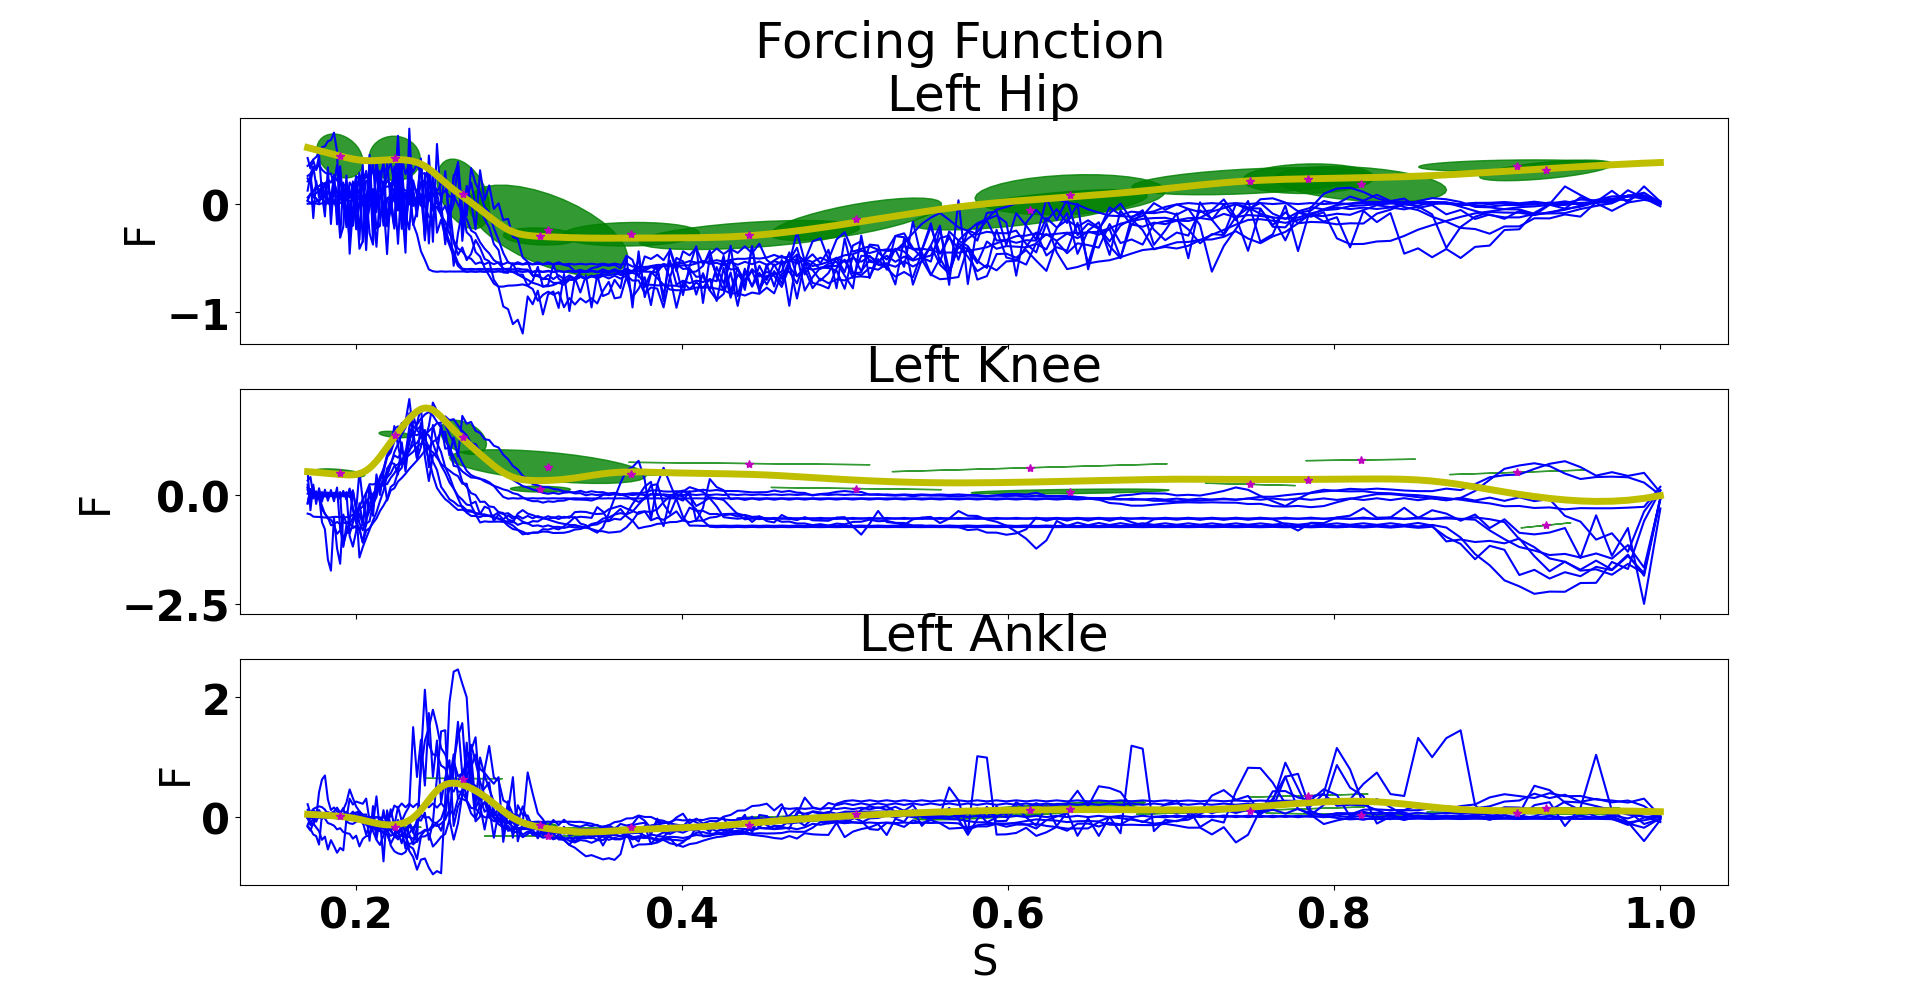
\includegraphics[scale=0.35]{images/gait_data/force_function2.png}
        \caption[Gait Forcing Function]{Forcing Function Learned for each of the trajectories. The red dots are the means and the green ovals are the covariances.}
        \label{fig:force}  
    \end{subfigure}

    \begin{subfigure}{\textwidth}
       \centering
    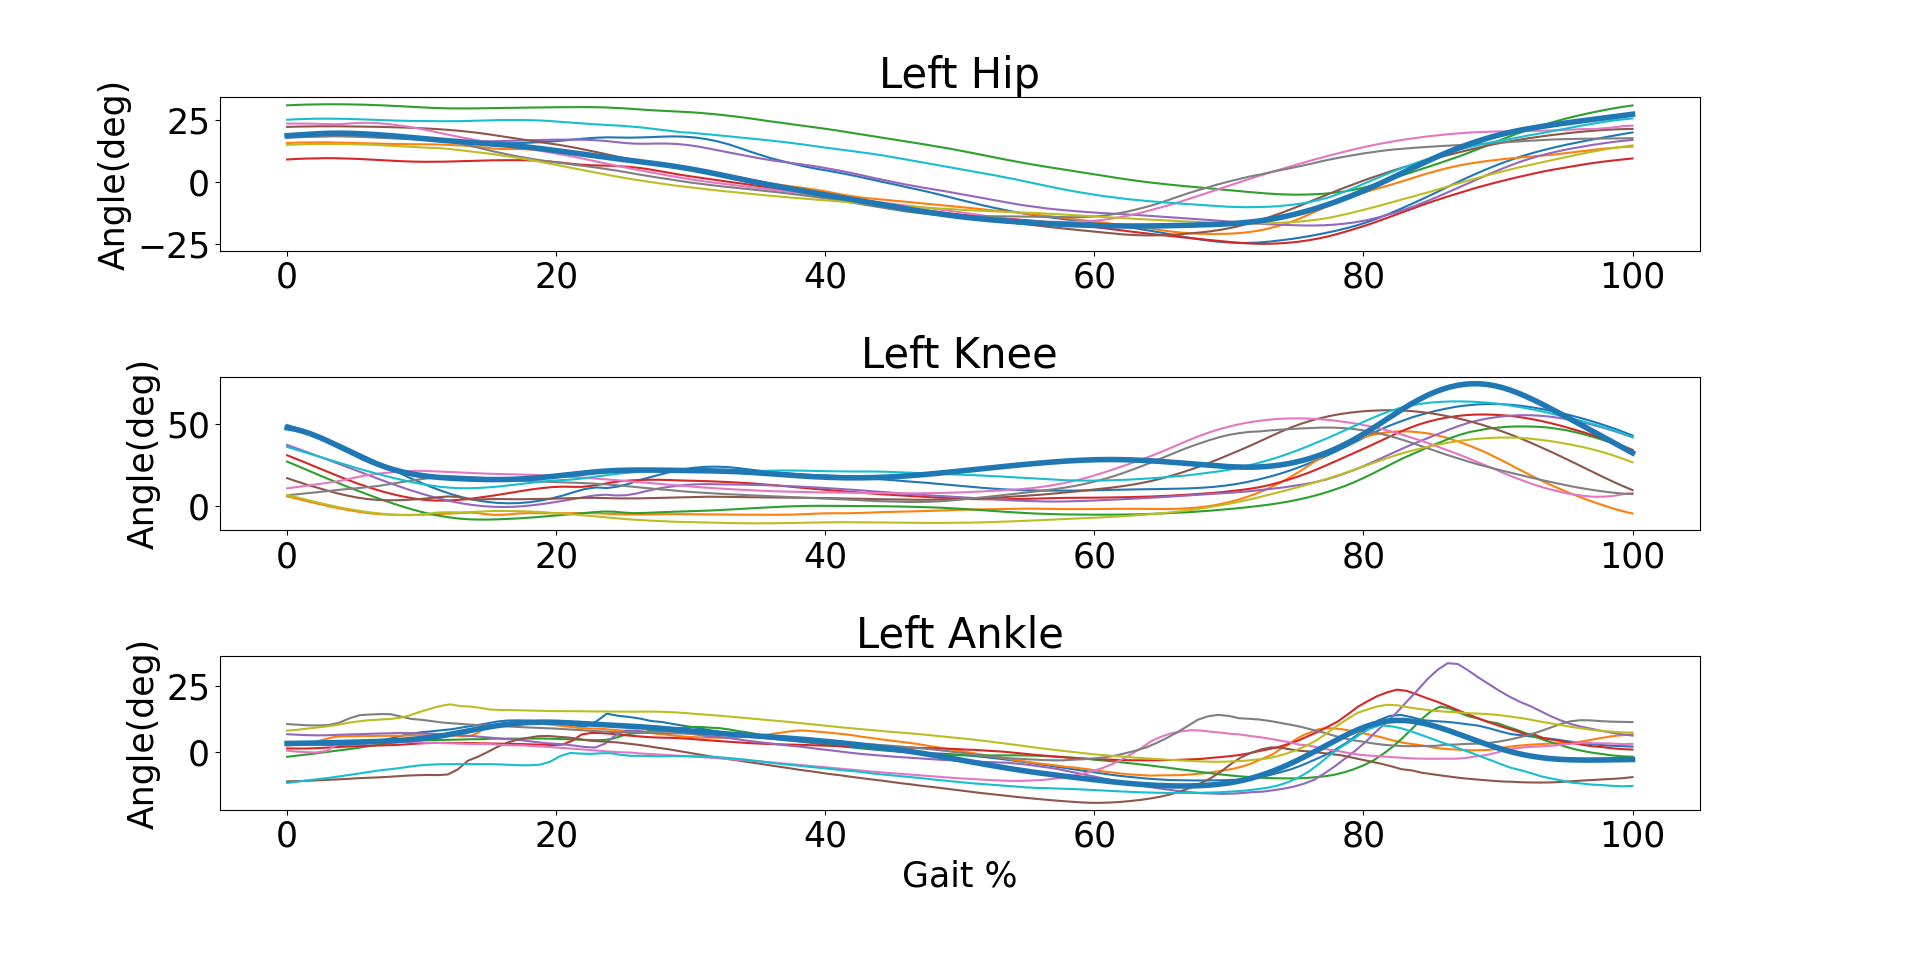
\includegraphics[scale=0.35]{images/gait_data/learnedModel.png}
    \caption[Learned Gait Model]{Learned model compared to the demonstrations. The thin lines are the demonstrations used to train the models. The thick line in the learned models.}
    \label{fig:learnedModel}
    \end{subfigure}
    \caption{Learning the gait trajectories}
    \label{fig:learninggaittrajectories}
\end{figure}





% \begin{figure}[h]
%     \centering
%     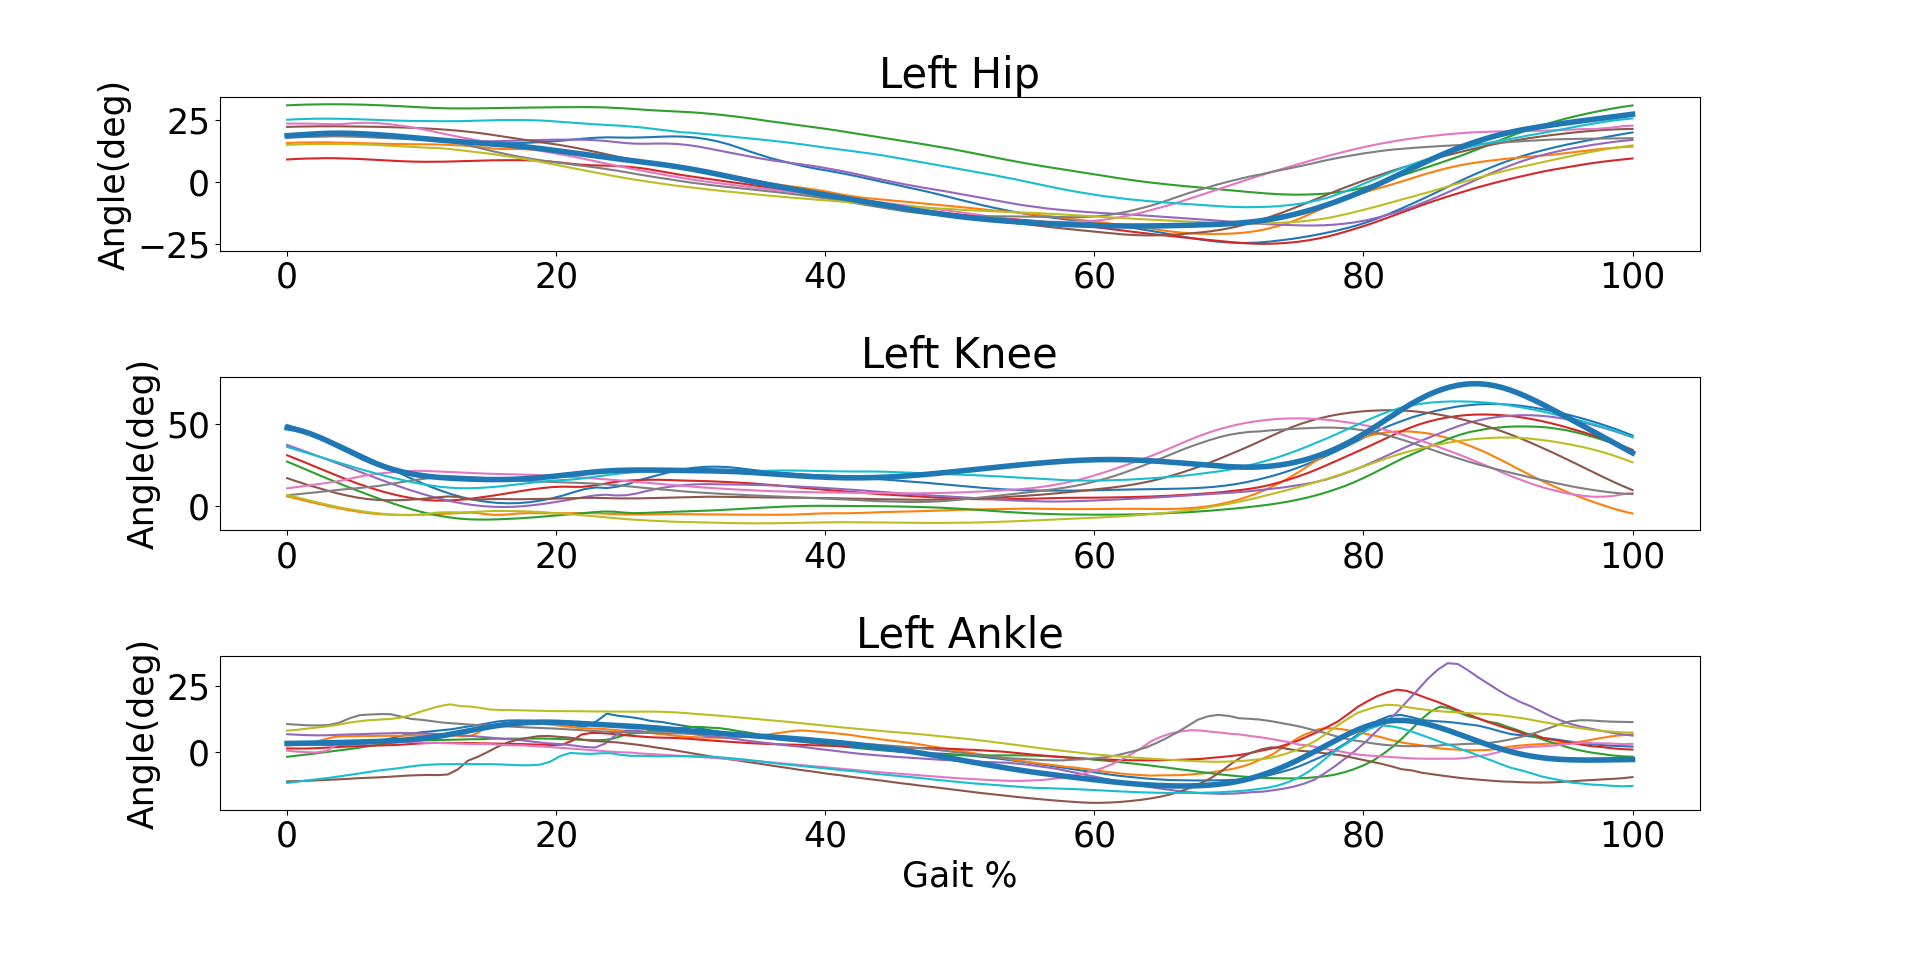
\includegraphics[scale=0.35]{images/gait_data/learnedModel.png}
%     \caption[Learned Gait Model]{Learned model compared to the demonstrations. The thin lines are the demonstrations used to train the models. The thick line in the learned models.}
%     \label{fig:learnedModel}
% \end{figure}

In addition to the learning the joint angles. The forward kinematics of the leg were record. This was done by using the marker on the toe as a training source. \autoref{fig:learnedToe} shows the forcing function and replicated gait motion using a marker placed on the toe of the subjects. The $Z$ and $X$ axis as referenced in \autoref{fig:TrainingJointPosition}. The $Y$ was not learned since the system is contrasted to the sagittal plane. In all four graphs the blue lines are the training demonstrations for the model. The green ovals in the upper two graphs are the Gaussians with the red dot being the mean. In the lower two graphs the black lines are replicated motion model. Using BIC it was detriment that 7 was the optimal number of bins to use. AS shown in \autoref{fig:FK_BIC}, 3-15 bins were test 10 times to ensure proper convergence. This ensured that a local minimization was found. In all but two iterations, the BIC score remained the identical. In the two remaining cases the BIC score of differed in the final bin size and does not effect the minimum BIC score.


\begin{figure}
    \centering
    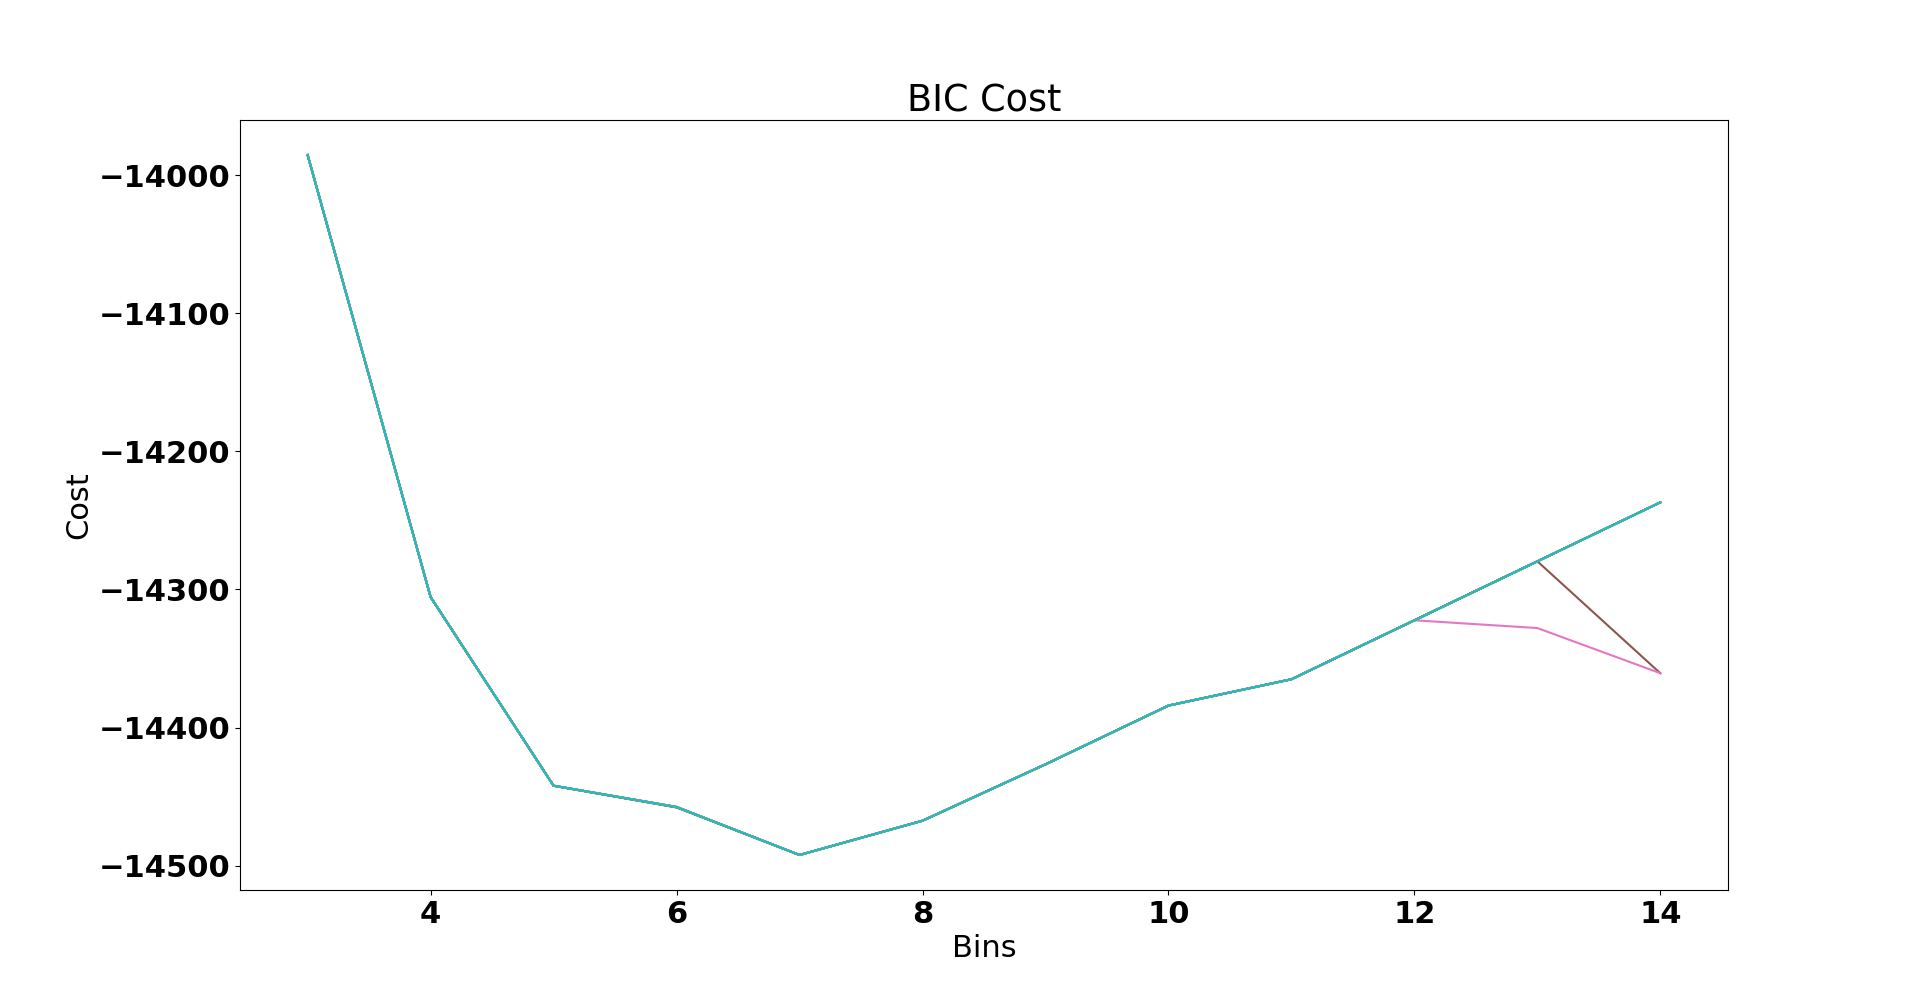
\includegraphics[scale=0.25]{images/gait_data/BIC_FK.png}
    \caption[FK BIC score]{BIC score for determining the optimal number of bins for learning the Fk position of the foot over a gait cycle}
    \label{fig:FK_BIC}
\end{figure}


\begin{figure}[!htb]
    \centering
    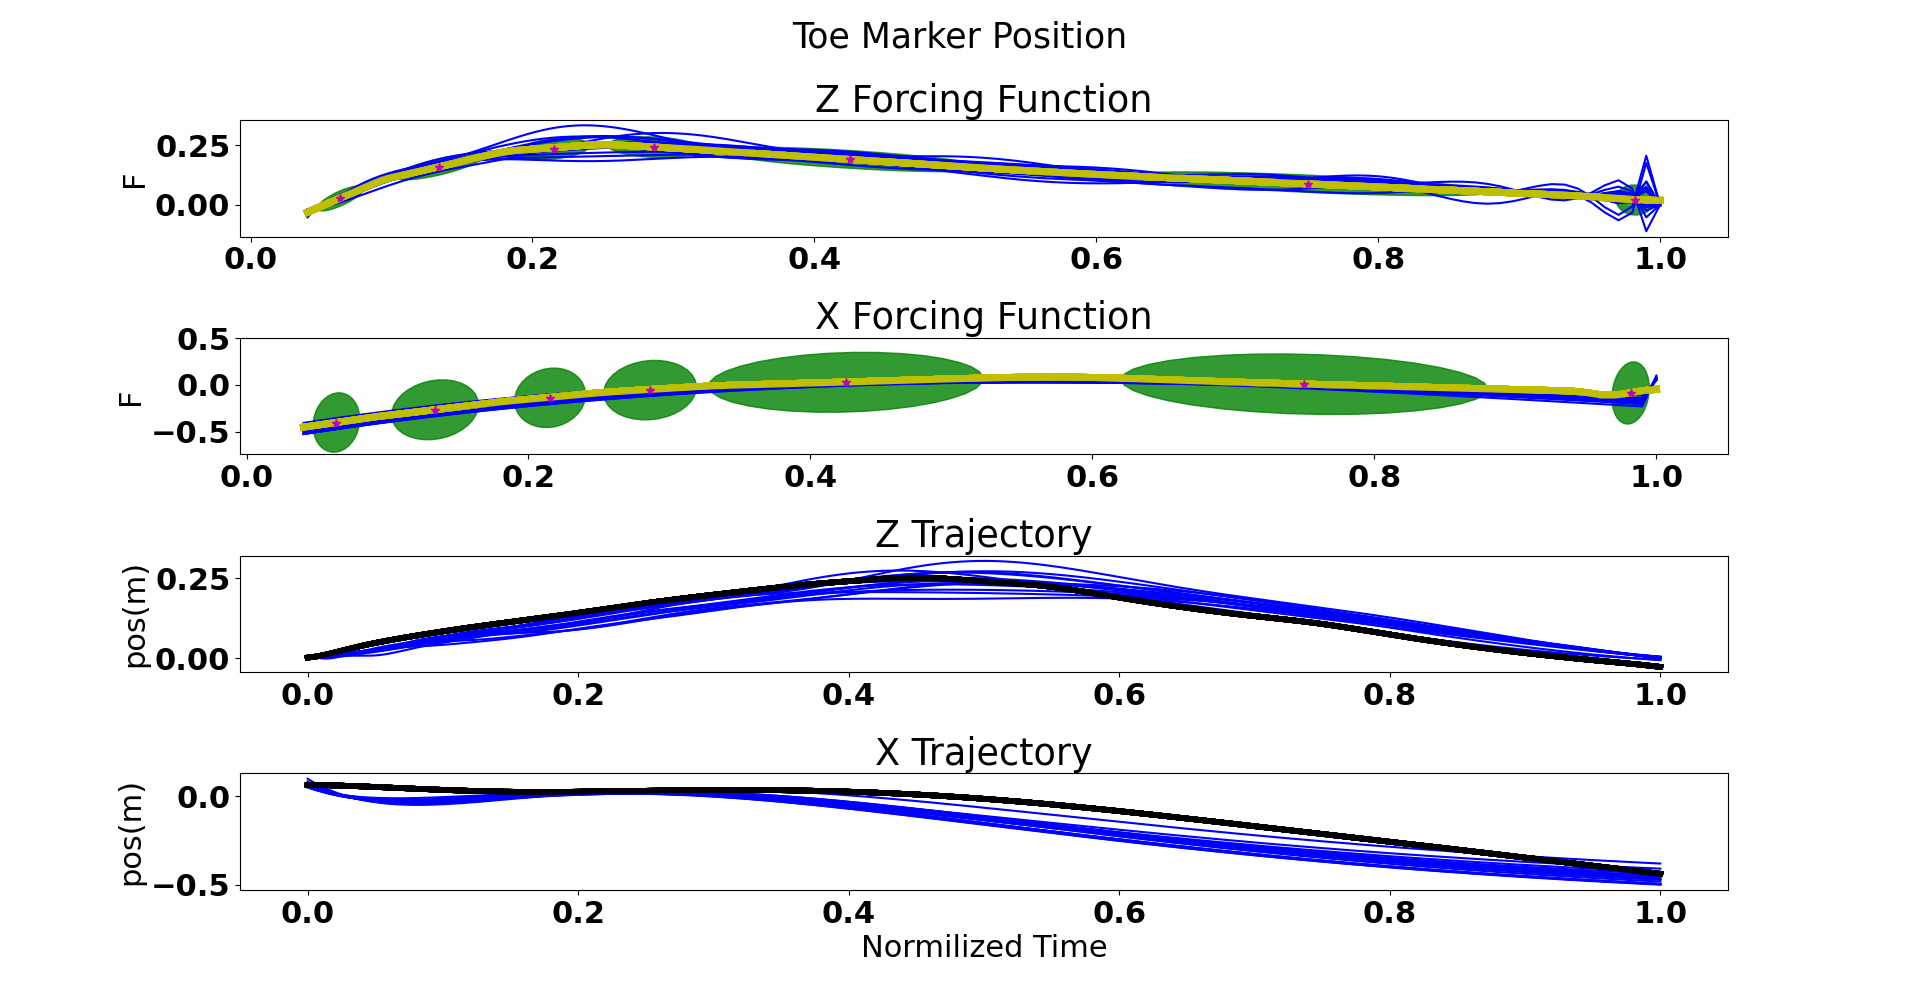
\includegraphics[scale=0.35]{images/gait_data/toe_maker_pos.png}
    \caption[Toe Marker Position]{Learning of the toe position during a single gait cycle, upper two graphs are the forcing functions. The lower two graphs are the replicated models an the training demonstrations.}
    \label{fig:learnedToe}
\end{figure}

Once the model is encoded using the tools discussed in \autoref{chap:software} can reproduce the joint trajectories. The processes to learn and reproduce the trajectories are separate systems allowing the encoding to be conducted offline and reproduced online. These models are used to generate the gait cycle for the exoskeleton in simulation. 


\section{Contributions}

All of the data collected was released open-source for community use and analysis. While there are other databases of gait motion out there, this data set provides additional information such as marker positions and joint torques. More markers and rigid bodies were used during the mocap trials than in past studies. The rigid bodies allow for analysis of leg segments relative motion. The raw marker position is valuable and can be used for observing the forward kinematics of the leg joints. 

Additionally, an extensive database of stair climbing motions was released. This open-source database contains all the kinematics information of how people of different ages, gender, heights climb stairs. This database helps study how people adjust to climbing stairs and help program robots to reproduce this motion. The trajectories can be encoded and reproduced on a human-robotic system. 

The collected information was used to learn motion models that replicated gait trajectories in both joint space and task space. Both of which were optimized using BIC. Using the BIC score the optimal number of bins were found to train the model. This generalized trajectories allows for varies type of controlled to be implemented. The generalized model will allow research's to have access to lower leg models to be used on there own exoskeletons or legged robotic systems. 